\tikzset{every picture/.style={line width=0.75pt}} %set default line width to 0.75pt        

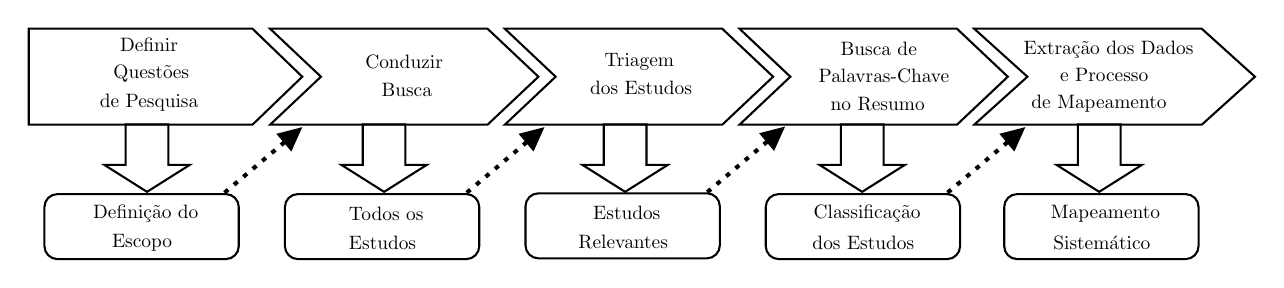
\begin{tikzpicture}[x=0.75pt,y=0.75pt,yscale=-1,xscale=1]
%uncomment if require: \path (0,295); %set diagram left start at 0, and has height of 295

%Pentagon Arrow [id:dp6278377926239387] 
\draw   (53.7,53) -- (161.5,53) -- (185.5,76.13) -- (161.5,99.25) -- (53.7,99.25) -- cycle ;
%Chevron Arrow [id:dp8061814950023936] 
\draw   (169.99,53) -- (274.76,53) -- (299.27,76.13) -- (274.76,99.25) -- (169.99,99.25) -- (194.5,76.13) -- cycle ;
%Chevron Arrow [id:dp5292331748785577] 
\draw   (283.07,53) -- (387.84,53) -- (412.35,76.13) -- (387.84,99.25) -- (283.07,99.25) -- (307.58,76.13) -- cycle ;
%Chevron Arrow [id:dp23027191263172608] 
\draw   (509.23,53) -- (618.86,53) -- (644.5,76.13) -- (618.86,99.25) -- (509.23,99.25) -- (534.87,76.13) -- cycle ;
%Chevron Arrow [id:dp12330558695774196] 
\draw   (396.15,53) -- (500.92,53) -- (525.42,76.13) -- (500.92,99.25) -- (396.15,99.25) -- (420.65,76.13) -- cycle ;
%Rounded Rect [id:dp4602302829049887] 
\draw   (61.27,138.93) .. controls (61.27,135.47) and (64.08,132.67) .. (67.54,132.67) -- (148.65,132.67) .. controls (152.11,132.67) and (154.91,135.47) .. (154.91,138.93) -- (154.91,157.73) .. controls (154.91,161.19) and (152.11,164) .. (148.65,164) -- (67.54,164) .. controls (64.08,164) and (61.27,161.19) .. (61.27,157.73) -- cycle ;
%Rounded Rect [id:dp8032081633216976] 
\draw   (523.69,138.93) .. controls (523.69,135.47) and (526.5,132.67) .. (529.96,132.67) -- (611.07,132.67) .. controls (614.53,132.67) and (617.33,135.47) .. (617.33,138.93) -- (617.33,157.73) .. controls (617.33,161.19) and (614.53,164) .. (611.07,164) -- (529.96,164) .. controls (526.5,164) and (523.69,161.19) .. (523.69,157.73) -- cycle ;
%Rounded Rect [id:dp3313220993143424] 
\draw   (408.8,138.93) .. controls (408.8,135.47) and (411.6,132.67) .. (415.06,132.67) -- (496.17,132.67) .. controls (499.63,132.67) and (502.44,135.47) .. (502.44,138.93) -- (502.44,157.73) .. controls (502.44,161.19) and (499.63,164) .. (496.17,164) -- (415.06,164) .. controls (411.6,164) and (408.8,161.19) .. (408.8,157.73) -- cycle ;
%Rounded Rect [id:dp4120899111688079] 
\draw   (293.04,138.57) .. controls (293.04,135.11) and (295.84,132.3) .. (299.3,132.3) -- (380.41,132.3) .. controls (383.87,132.3) and (386.68,135.11) .. (386.68,138.57) -- (386.68,157.37) .. controls (386.68,160.83) and (383.87,163.64) .. (380.41,163.64) -- (299.3,163.64) .. controls (295.84,163.64) and (293.04,160.83) .. (293.04,157.37) -- cycle ;
%Rounded Rect [id:dp45930303754942536] 
\draw   (177.13,138.93) .. controls (177.13,135.47) and (179.94,132.67) .. (183.4,132.67) -- (264.5,132.67) .. controls (267.97,132.67) and (270.77,135.47) .. (270.77,138.93) -- (270.77,157.73) .. controls (270.77,161.19) and (267.97,164) .. (264.5,164) -- (183.4,164) .. controls (179.94,164) and (177.13,161.19) .. (177.13,157.73) -- cycle ;
%Down Arrow [id:dp3807248413929003] 
\draw  [line width=0.75]  (90.13,118.6) -- (100.42,118.6) -- (100.42,99.1) -- (121,99.1) -- (121,118.6) -- (131.3,118.6) -- (110.71,131.6) -- cycle ;
%Down Arrow [id:dp47792969981808375] 
\draw  [line width=0.75]  (204.34,118.6) -- (214.63,118.6) -- (214.63,99.1) -- (235.21,99.1) -- (235.21,118.6) -- (245.5,118.6) -- (224.92,131.6) -- cycle ;
%Down Arrow [id:dp6527476506757643] 
\draw  [line width=0.75]  (320.47,118.6) -- (330.76,118.6) -- (330.76,99.1) -- (351.34,99.1) -- (351.34,118.6) -- (361.63,118.6) -- (341.05,131.6) -- cycle ;
%Down Arrow [id:dp6109879640313591] 
\draw  [line width=0.75]  (434.68,118.6) -- (444.97,118.6) -- (444.97,99.1) -- (465.55,99.1) -- (465.55,118.6) -- (475.84,118.6) -- (455.26,131.6) -- cycle ;
%Down Arrow [id:dp08052269206416462] 
\draw  [line width=0.75]  (548.88,118.6) -- (559.17,118.6) -- (559.17,99.1) -- (579.75,99.1) -- (579.75,118.6) -- (590.04,118.6) -- (569.46,131.6) -- cycle ;
%Straight Lines [id:da6425776226592788] 
\draw [line width=1.5]  [dash pattern={on 1.69pt off 2.76pt}]  (148.07,132) -- (183.21,102.37) ;
\draw [shift={(185.5,100.43)}, rotate = 499.86] [fill={rgb, 255:red, 0; green, 0; blue, 0 }  ][line width=1.5]  [draw opacity=0] (11.61,-5.58) -- (0,0) -- (11.61,5.58) -- cycle    ;

%Straight Lines [id:da624041708353656] 
\draw [line width=1.5]  [dash pattern={on 1.69pt off 2.76pt}]  (264.75,132) -- (299.89,102.37) ;
\draw [shift={(302.18,100.43)}, rotate = 499.86] [fill={rgb, 255:red, 0; green, 0; blue, 0 }  ][line width=1.5]  [draw opacity=0] (11.61,-5.58) -- (0,0) -- (11.61,5.58) -- cycle    ;

%Straight Lines [id:da30892482975542945] 
\draw [line width=1.5]  [dash pattern={on 1.69pt off 2.76pt}]  (380.65,131.73) -- (415.79,102.1) ;
\draw [shift={(418.09,100.16)}, rotate = 499.86] [fill={rgb, 255:red, 0; green, 0; blue, 0 }  ][line width=1.5]  [draw opacity=0] (11.61,-5.58) -- (0,0) -- (11.61,5.58) -- cycle    ;

%Straight Lines [id:da19825567767990848] 
\draw [line width=1.5]  [dash pattern={on 1.69pt off 2.76pt}]  (496.41,132) -- (531.56,102.37) ;
\draw [shift={(533.85,100.43)}, rotate = 499.86] [fill={rgb, 255:red, 0; green, 0; blue, 0 }  ][line width=1.5]  [draw opacity=0] (11.61,-5.58) -- (0,0) -- (11.61,5.58) -- cycle    ;


% Text Node
\draw (111.66,60.53) node [scale=0.7] [align=left] {Definir};
% Text Node
\draw (112.75,74.83) node [scale=0.7] [align=left] {Questões};
% Text Node
\draw (111.66,88.6) node [scale=0.7] [align=left] {de Pesquisa};
% Text Node
\draw (234.55,68.76) node [scale=0.7] [align=left] {Conduzir};
% Text Node
\draw (235.84,82.37) node [scale=0.7] [align=left] {Busca};
% Text Node
\draw (347.88,68.76) node [scale=0.7] [align=left] {Triagem};
% Text Node
\draw (348.71,81.64) node [scale=0.7] [align=left] {dos Estudos};
% Text Node
\draw (463.25,62.65) node [scale=0.7] [align=left] {Busca de};
% Text Node
\draw (465.75,75.78) node [scale=0.7] [align=left] {Palavras-Chave};
% Text Node
\draw (462.75,89.1) node [scale=0.7] [align=left] {no Resumo};
% Text Node
\draw (573.99,63) node [scale=0.7] [align=left] {Extração dos Dados};
% Text Node
\draw (571.87,75.27) node [scale=0.7] [align=left] {e Processo};
% Text Node
\draw (569.37,89.19) node [scale=0.7] [align=left] {de Mapeamento};
% Text Node
\draw (110.09,142.14) node [scale=0.7] [align=left] {Definição do};
% Text Node
\draw (108.31,155.98) node [scale=0.7] [align=left] {Escopo};
% Text Node
\draw (572.51,142.14) node [scale=0.7] [align=left] {Mapeamento};
% Text Node
\draw (570.74,155.98) node [scale=0.7] [align=left] {Sistemático};
% Text Node
\draw (457.62,142.14) node [scale=0.7] [align=left] {Classificação};
% Text Node
\draw (455.84,155.98) node [scale=0.7] [align=left] {dos Estudos};
% Text Node
\draw (341.85,141.77) node [scale=0.7] [align=left] {Estudos};
% Text Node
\draw (340.08,155.62) node [scale=0.7] [align=left] {Relevantes};
% Text Node
\draw (225.95,142.14) node [scale=0.7] [align=left] {Todos os};
% Text Node
\draw (224.17,155.98) node [scale=0.7] [align=left] {Estudos};


\end{tikzpicture}